% =====================================================================================================
%  main2.tex: point-form summary of the work.
%  Sections: novelty (with proof), faults considered, variations of each stage, fault-type groups,
%  fault detection, winning (proposed vs MENDNet vs SDN), architecture and results.
%  Numbers: main.tex / stage2_paper/results/paper/paper_tables.md; over-confidence table from
%  overconfidence_check.py (stored final-model logits, results/campaigns/final).
% =====================================================================================================
\documentclass[10pt,a4paper]{article}

\usepackage[utf8]{inputenc}
\usepackage[T1]{fontenc}
\usepackage{lmodern}
\usepackage[margin=2.2cm]{geometry}
\usepackage{amsmath,amssymb}
\usepackage{booktabs}
\usepackage{float}
\usepackage{adjustbox}
\usepackage{enumitem}
\usepackage{xcolor}
\usepackage{tikz}
\usetikzlibrary{positioning,arrows.meta}
\usepackage{hyperref}
\setlist{itemsep=1pt,topsep=2pt}

\newcommand{\meth}[1]{\texttt{#1}}
\newcommand{\ours}{\meth{margin\_band}}
\definecolor{cours}{HTML}{1F6FB2}

\title{Early Exits for Weight-Memory Fault Detection and Tolerance:\\
Calibrated Logit Bands Against Silent Data Corruption in CNNs\\[4pt]
\large Summary in points}
\author{TODO: authors}
\date{}

\begin{document}
\maketitle

% -----------------------------------------------------------------------------------------------------
\section{Novelty}

\begin{itemize}
  \item \textbf{Not new (building blocks, cited):} early exit on the margin (big/little networks); max logit as a
        score (MaxLogit); range checks / clipping against hardware faults (Li et al.\ 2017, Ranger, FT-ClipAct).
  \item \textbf{New, with respect to MENDNet (DAC 2024):}
  \begin{enumerate}
    \item \textbf{Finding: weight-memory faults make the network \emph{over}-confident, not uncertain.}
          Proof below (Table~\ref{tab:overconf}).
    \item \textbf{Two-sided max-logit band} at every exit and at the final classifier, \textbf{calibrated on clean
          data only} with a false-alarm budget $\alpha$. MENDNet tunes its thresholds on fault-injected data.
    \item \textbf{One set of exits, two jobs:} margin $\to$ early exit ($60.5\,\%$ FLOPs saved); band $\to$
          fault detection (SDC $13.4 \to 0.223\,\%$).
    \item \textbf{Exit architecture by multi-objective NAS}, every step validated. MENDNet uses fixed exits.
    \item \textbf{Fair evaluation:} all methods on the same stored faulty logits; MENDNet with clean and with
          faulty-data calibration; three fault models; run-level statistics; measured latency.
    \item \textbf{Low-Overhead decision:} top-2 comparator tree, 1 subtraction, 3 comparisons per exit; no exp, log,
          division.
  \end{enumerate}
\end{itemize}

\subsection*{Proof that faults increase confidence}

\begin{itemize}
  \item \textbf{Test:} every image the plain network answers correctly when clean and \emph{wrongly} under the
        fault (an SDC); FP32 exponent faults, G1--G3, $k=1..8$, final model; \textbf{3.97\,M SDC images}.
  \item \textbf{Compared with:} the clean validation distribution of the final classifier (max logit 0.5\,/\,99.5
        percentile $= 3.57\,/\,9.58$, median $8.66$; MSP 1st percentile $0.57$).
  \item \textbf{Finiteness:} the logits come from the same campaign, so the finiteness check was already applied
        at injection time (faults giving Inf/NaN redrawn). Re-checked on the stored data: all
        $1.28\cdot10^{9}$ stored logit values (32 files, all groups and $k$) are finite; the largest $|$logit$|$ is
        $3.03\cdot10^{38}$, just below the FP32 maximum $3.40\cdot10^{38}$. The over-confidence is therefore
        measured on finite, plausible-looking outputs only, not on Inf/NaN.
\end{itemize}

\begin{table}[H]
\centering\small
\caption{Faulty outputs of SDC images vs the clean distribution (plain network, final classifier). Only faults
that pass the finiteness check (all logits finite) are included.}
\label{tab:overconf}
\begin{adjustbox}{max width=\linewidth}
\begin{tabular}{@{}lrrrrr@{}}
\toprule
SDC images & Count & Max logit $>$ clean 99.5th & Max logit $<$ clean 0.5th & MSP $<$ clean 1st pct & Median max logit \\
\midrule
clean reference                 & ---        & ---              & ---    & ---    & 8.66 \\
\textbf{all, G1--G3}            & 3{,}966{,}176 & \textbf{99.2\,\%} & 0.1\,\% & 0.2\,\% & $\mathbf{2.2\cdot10^{34}}$ \\
runs with a bit-30 flip         & 3{,}947{,}379 & 99.7\,\% & 0.0\,\% & 0.1\,\% & $2.2\cdot10^{34}$ \\
runs without bit 30             & 18{,}797   & 0.0\,\%  & 12.1\,\% & 28.7\,\% & 4.99 \\
G1 / G2 / G3                    & 1.15 / 1.61 / 1.21\,M & 97.9 / 99.5 / 100\,\% & $\le 0.2\,\%$ & $\le 0.6\,\%$ & $\sim 10^{34}$ \\
\bottomrule
\end{tabular}
\end{adjustbox}
\end{table}

\begin{itemize}
  \item \textbf{99.2\,\%} of silent corruptions have a max logit \emph{above} anything seen on clean data
        (median $10^{34}$ vs $8.66$); only $0.1$--$0.2\,\%$ are in the low tail.
  \item The negative energy gives the same picture: $99.2\,\%$ $\ge$ clean median, $0.1\,\%$ below clean 1st pct.
  \item \textbf{Consequence:} low-confidence detectors (MSP, energy, MENDNet) inspect the wrong tail
        $\Rightarrow$ detection ratio $<1\,\%$, run TPR $<5\,\%$.
  \item \textbf{Ablation confirms it:} lower bound only: SDC $7.93\,\%$ ($=$ no band $7.95\,\%$);
        upper bound only: SDC $0.194\,\%$ ($97.6\,\%$ removed); both: $0.143\,\%$.
  \item \textbf{Cause:} bit 30 multiplies a typical weight ($|w|<2$) by $2^{128}$; bit-30 runs give
        $99.5\,\%$ of all SDC images.
  \item \textbf{Qualifier:} the rare SDCs without bit 30 ($0.5\,\%$) are \emph{under}-confident; the lower side of
        the band is for them. Under MENDNet's sign-flip faults logits shrink/scramble, so the finding is specific
        to exponent faults.
\end{itemize}

% -----------------------------------------------------------------------------------------------------
\section{Faults considered: no NaN / Inf}

\begin{itemize}
  \item \textbf{Faults giving Inf or NaN are excluded:} any fault that makes a weight or a logit non-finite is
        rejected and redrawn.
  \item \textbf{When the check is done:} at injection time, \emph{before} any method is evaluated. Each drawn
        fault is applied; if the weight, or any logit of any exit or of the final classifier on any of the
        10{,}000 test images, is non-finite, the fault is undone and a new one is drawn. The check is repeated
        after every added fault, so the $k$ faults of a run are finite \emph{together}. Only then are the logits
        stored, and all methods are evaluated offline on these finite logits.
  \item \textbf{Why:} a non-finite output is caught by a trivial finiteness check, so it is not \emph{silent}.
        Only finite, plausible-looking outputs are hard to detect.
  \item \textbf{How many:} 136 of 14{,}536 drawn faults ($0.94\,\%$) were rejected, all bit-30 flips, all due to
        non-finite logits; 130 of 3{,}200 runs needed a redraw (G1 33, G2 11, G3 10, HEADS 82 draws).
  \item \textbf{Effect:} every reported SDC comes from a finite output; reported numbers are the hard case
        (counting non-finite faults as detected would only make all band rules look better).
\end{itemize}

% -----------------------------------------------------------------------------------------------------
\section{Each stage: what was explored}

\subsection{Stage A: exit condition}

\begin{itemize}
  \item \textbf{Exit score (when to leave early), types explored:}
  \begin{itemize}
    \item max softmax probability (SDN, MSP);
    \item negative energy (log-sum-exp);
    \item MENDNet Algorithm~1 (energy with $\gamma,\tau$);
    \item max logit;
    \item \textbf{margin = top-1 $-$ top-2 logit (chosen)};
    \item margin + agreement with the next exit.
  \end{itemize}
  \item \textbf{Acceptance gate / detector, types explored:}
  \begin{itemize}
    \item none (SDN);
    \item one-sided low threshold (MSP-low, energy-low, MENDNet $\tau$);
    \item \textbf{two-sided band on max logit (chosen)};
    \item two-sided band on energy;
    \item multi-band on max, min and sum of logits.
  \end{itemize}
  \item \textbf{Band sides:} none / lower only / upper only / \textbf{both}.
  \item \textbf{Calibration data:} \textbf{clean validation (ours)} vs fault-injected validation (MENDNet).
  \item \textbf{Calibration slack} (accuracy loss allowed per exit): 0 / \textbf{0.5} / 1 point.
  \item \textbf{False-alarm budget $\alpha$:} 0.25 / 0.5 / \textbf{1} / 2 / 5 / 10\,\%.
  \item \textbf{Outcome (SDC / FLOPs saved / run TPR):}
  \begin{itemize}
    \item \ours: $0.223\,\%$ / $\mathbf{60.5\,\%}$ / $93.1\,\%$ $\leftarrow$ chosen, best trade-off;
    \item \meth{margin\_multiband}: $0.212$ / $60.4$ / $93.8$ (more operations, no gain);
    \item \meth{maxlogit\_band}: $0.181$ / $55.5$ / $92.5$;
    \item \meth{energy\_band}: $0.181$ / $55.3$ / $85.6$ (needs exp, log);
    \item \meth{margin\_band\_agree}: $0.174$ / $48.9$ / $97.1$ (computes next exit, less saving);
    \item slack 0: SDC $0.107\,\%$ but saved only $36.9\,\%$; $\alpha=0.25\,\%$ already works (SDC $0.233\,\%$);
          TPR drops at $\alpha\ge5\,\%$.
  \end{itemize}
\end{itemize}

\subsection{Stage B: NAS (exit placement and head architecture)}

\begin{itemize}
  \item \textbf{Searched per exit:} position (17 candidates); number of exits $K\in\{1,2,3\}$; conv blocks
        $n\in\{0,1,2\}$; conv type std / depthwise-separable; channel ratio $r\in\{1/2,1/4,1/8\}$; pooling
        $q\in\{1,2,4\}$; hidden FC $\in\{0,64,128,256\}$; rule \ours\ / \meth{maxlogit\_band}.
  \item \textbf{Objectives:} max accuracy, min expected FLOPs, min head parameters; constraint accuracy
        $\ge$ backbone $-1$. Thresholds always calibrated, never searched.
  \item \textbf{All search methods that were run:}
  \begin{enumerate}
    \item \textbf{Stage-0 random search (original project):} 300 random configurations (1--3 exits, random
          positions, heads from a fixed menu A1--A5, \emph{random} margin thresholds in $[1,4]$); pick by a weighted
          score (FLOPs saved $-\,2\times$ head overhead, accuracy $\ge$ backbone $-1$) $\Rightarrow$ exits
          \textbf{16/23} (heads A4, A3), the \meth{old1623} model. Replaced because thresholds were searched instead
          of calibrated and a single weighted score hides the trade-off.
    \item \textbf{Hand-placed designs} (no search): 6/13/23 with default heads; 16/23 kept as reference.
    \item \textbf{Multi-objective samplers}, same full space, 250 trials, 3 seeds each (Optuna):
          TPE (multivariate), NSGA-II (population 50), random search.
    \item \textbf{Restricted search spaces} (TPE): fixed head menu A1--A5; positions only (default head);
          heads only (positions fixed 16, 23).
    \item \textbf{Fixed number of exits} (TPE): exactly 1, exactly 2, exactly 3.
    \item \textbf{Fixed rule} (TPE): rule fixed to \ours; fixed to \meth{maxlogit\_band}.
    \item \textbf{Fault-aware objectives} (TPE): + head-fault SDC from a 40-fault probe (4 objectives);
          head params replaced by exposure.
    \item \textbf{Pick rules on the Pareto front:} P1 lowest FLOPs; P2 fewest head params; P3 lowest head-fault
          SDC (with saving $\ge$ the 16/23 model); P4 lowest FLOPs with exactly 2 exits; \textbf{final:} top-5
          lowest-FLOPs points fully trained, lowest FLOPs with VAL\_SEL acc $\ge 91.84\,\%$.
  \end{enumerate}
\end{itemize}

\begin{table}[H]
\centering\small
\caption{Search methods compared: hypervolume (HV, common reference point; accuracy, expected FLOPs, head
parameters), 3 sampler seeds (1 for D1/D2). Best feasible = lowest expected MFLOPs with accuracy $\ge$
backbone $-1$ (backbone 627.9 MFLOPs).}
\begin{adjustbox}{max width=\linewidth}
\begin{tabular}{@{}llrrrr@{}}
\toprule
Variant & Method / search space & HV & Pareto pts & Best feasible MFLOPs & Wall (min) \\
\midrule
A1 & \textbf{TPE, full space}             & $\mathbf{7.04\pm0.45}$ & 63.3 & 315 & 10.5 \\
A2 & NSGA-II, full space                  & $6.25\pm0.14$ & 33.7 & 321 & 7.6 \\
A3 & random search, full space            & $6.23\pm0.28$ & 36.3 & 318 & 11.8 \\
B1 & TPE, fixed head menu A1--A5          & $6.18\pm0.17$ & 72.0 & 335 & 0.9 \\
B2 & TPE, positions only                  & $5.14\pm0.10$ & 103  & 327 & 0.1 \\
B3 & TPE, heads only (16, 23)             & $6.77\pm0.20$ & 68.3 & 306 & 0.2 \\
C1 / C2 / C3 & TPE, exactly 1 / 2 / 3 exits & $6.01$ / $6.76$ / $6.88$ & 63 / 57 / 34 & 342 / 314 / 308 & 1.0 / 2.1 / 1.6 \\
D1 / D2 & TPE, rule fixed \ours\ / \meth{maxlogit\_band} & $6.25$ / $6.60$ & 54 / 69 & 324 / 328 & 1.1 / 0.7 \\
E1 & TPE, + head-fault SDC objective      & $6.68\pm0.27$ & 54.0 & 310 & 19.0 \\
E2 & TPE, exposure instead of params      & $7.00\pm0.23$ & 34.7 & 298 & 19.1 \\
\bottomrule
\end{tabular}
\end{adjustbox}
\end{table}

\begin{itemize}
  \item \textbf{What the comparison shows:}
  \begin{itemize}
    \item \textbf{TPE is the best sampler} ($7.04$), clearly above NSGA-II ($6.25$) and random search ($6.23$)
          with the same budget;
    \item searching \textbf{positions and heads together} matters: positions only is the worst ($5.14$), a fixed
          menu is also worse ($6.18$);
    \item up to 3 exits beats a single exit ($6.88$ vs $6.01$);
    \item fault-aware objectives do not raise the HV $\Rightarrow$ keep fault detection in the calibrated rule,
          not in the search;
    \item stage-0 random search with searched thresholds gave 16/23: $52.5\,\%$ saved, $1.10$\,M head params;
          the final TPE model: $60.5\,\%$ saved, $0.26$\,M head params ($4\times$ fewer), similar SDC.
  \end{itemize}
  \item \textbf{Validation of each step:}
  \begin{itemize}
    \item proxy 4 / \textbf{8} / 16 epochs vs full 60: Spearman $0.988$ / $\mathbf{0.987}$ / $0.995$;
    \item fault probe (40 faults) vs full campaign (200): $\rho=0.875$, $p=9\cdot10^{-4}$;
    \item searched vs hand-placed: $50$--$51\,\%$ vs $40$--$46\,\%$ saved, $3$--$4.5\times$ fewer head params;
    \item NAS vs hand 16/23 under faults: significant but tiny SDC difference $\Rightarrow$ protection comes from
          the band;
    \item full training of top candidates changes the ranking: best proxy $54.0\,\%$ saved, \meth{s11\_t229}
          $\mathbf{60.8\,\%}$ $\Rightarrow$ final model.
  \end{itemize}
\end{itemize}

% -----------------------------------------------------------------------------------------------------
\section{Fault-type groups}

\begin{itemize}
  \item \textbf{Main fault model:} FP32 weight memory, one random exponent bit (23--30) in each of $k=1..8$
        distinct random weights, persistent, 100 runs per (group, $k$) $=3{,}200$ runs $\times$ 10{,}000 images.
  \item \textbf{Groups (where the faulty weights are drawn):}
  \begin{itemize}
    \item \textbf{G1:} backbone before the first exit ($f_0..f_{13}$);
    \item \textbf{G2:} backbone between the first and the last exit ($f_{14}..f_{26}$);
    \item \textbf{G3:} backbone after the last exit + classifier ($f_{27}..f_{43}$, FC);
    \item \textbf{HEADS:} the exit heads.
  \end{itemize}
  \item \textbf{SDC per group (plain / SDN / MENDNet-clean / ours, \%):}
  \begin{itemize}
    \item G1: $15.6$ / $16.0$ / $15.8$ / $\mathbf{0.621}$ (hardest: every exit sees corrupted features);
    \item G2: $21.8$ / $2.65$ / $4.98$ / $\mathbf{0.089}$;
    \item G3: $16.4$ / $0.736$ / $0.952$ / $\mathbf{0.002}$ (early exit avoids most of it);
    \item HEADS: $0$ / $5.79$ / $7.62$ / $\mathbf{0.179}$ (plain has no heads).
  \end{itemize}
  \item \textbf{Other fault models:}
  \begin{itemize}
    \item \textbf{MENDNet groups (sign flips of FR $=10/30/50\,\%$):} FP1 final classifier (ours best, SDC 0),
          FP2 exit-2 head and FP3 first conv after exit 1 (MENDNet-faulty often better), FP4 first conv (all fail);
    \item \textbf{INT8} (simulated weight-only): faults nearly harmless for all methods (SDC $\le0.02\,\%$).
  \end{itemize}
\end{itemize}

% -----------------------------------------------------------------------------------------------------
\section{Fault detection: energy and the other detectors}

\begin{itemize}
  \item \textbf{Metrics:} per image: SDC rate, detection ratio = flagged / (flagged + SDC); per run: binomial
        test vs clean FAR ($p<0.01$), TPR on harmful runs, FPR on harmless runs, images until detection.
  \item \textbf{One-sided (low-confidence) detectors fail:}
  \begin{itemize}
    \item MSP-low: SDC $6.23\,\%$, det.\ ratio $0.57\,\%$, TPR $3.5\,\%$;
    \item \textbf{energy-low:} SDC $7.14\,\%$, det.\ ratio $0.34\,\%$, TPR $4.8\,\%$;
    \item MENDNet-clean: SDC $7.35\,\%$, det.\ ratio $0.34\,\%$, TPR $4.8\,\%$;
    \item MENDNet-faulty-val: threshold falls to zero flags, detects nothing;
    \item larger $\alpha$ does not help (MENDNet SDC $7.0 \to 11.0\,\%$ from $\alpha=0.25$ to $10\,\%$).
  \end{itemize}
  \item \textbf{Two-sided bands work:}
  \begin{itemize}
    \item \textbf{ours:} SDC $\mathbf{0.223\,\%}$, det.\ ratio $95.9\,\%$, TPR $\mathbf{93.1\,\%}$, FPR $0.08\,\%$,
          200 images to detect;
    \item \textbf{energy-band:} SDC $0.181\,\%$, det.\ ratio $97.0\,\%$, TPR $85.6\,\%$, FPR $0.34\,\%$;
    \item max-logit band: SDC $0.181\,\%$, TPR $92.5\,\%$, FPR $0.51\,\%$.
  \end{itemize}
  \item \textbf{So:} the score matters less than the \emph{upper} bound; energy works once it is two-sided.
\end{itemize}

% -----------------------------------------------------------------------------------------------------
\section{Winning: proposed vs MENDNet vs SDN}

\begin{table}[H]
\centering\small
\caption{Final model, FP32 exponent faults, $k=1..8$, all groups, 3{,}200 runs $\times$ 10{,}000 images.}
\begin{adjustbox}{max width=\linewidth}
\begin{tabular}{@{}lrrrrrrrr@{}}
\toprule
Method & Clean acc. & FAR & FLOPs saved & \textbf{SDC} & Det.\ ratio & Run TPR & Acc.\ under faults & with fallback \\
 & \% & \% & \% & \% & \% & \% & \% & \% \\
\midrule
Plain VGG16 (no exits)          & 92.3 & 0    & 0    & 13.4  & 0    & 0    & 80.0 & 80.0 \\
SDN (\meth{sdn\_msp})           & 91.8 & 0    & 60.0 & 6.30  & 0    & 0    & 86.2 & 86.2 \\
MENDNet, clean calib.           & 91.6 & 1.12 & 54.3 & 7.35  & 0.34 & 4.8  & 85.0 & 85.3 \\
MENDNet, faulty-val calib.      & 91.2 & 0    & 61.2 & 6.12  & 0    & 0    & 85.8 & 85.8 \\
\midrule
\textbf{Proposed (\ours)}       & 91.2 & 0.95 & 60.5 & \textbf{0.223} & \textbf{95.9} & \textbf{93.1} & \textbf{86.4} & \textbf{87.4} \\
\bottomrule
\end{tabular}
\end{adjustbox}
\end{table}

\begin{itemize}
  \item \textbf{vs SDN:} same saving ($60.5$ vs $60.0\,\%$); SDN detects nothing; SDC $6.30 \to 0.223\,\%$
        ($28\times$ lower).
  \item \textbf{vs MENDNet:} SDC $7.35 \to 0.223\,\%$ ($33\times$); run TPR $4.8 \to 93.1\,\%$; no fault data;
        no exp/log/division.
  \item \textbf{vs plain:} SDC $13.4 \to 0.223\,\%$ ($60\times$).
  \item \textbf{Tolerance} (share of the 12.3-point loss recovered): plain 0, MENDNet 43--47, SDN 50,
        \textbf{ours 60\,\%} $\Rightarrow$ partial.
  \item \textbf{Cost:} $-1.1$ points clean accuracy, $0.95\,\%$ clean false alarms.
  \item \textbf{Where it does not win} (reported honestly):
  \begin{enumerate}
    \item \textbf{MENDNet's own fault model, groups FP2 and FP3.} This model flips the \emph{sign} bit of
          FR $=10/30/50\,\%$ of the weights of one group: FP1 final classifier, FP2 exit-2 head,
          FP3 first conv after exit 1, FP4 first conv.
    \begin{itemize}
      \item Sign flips \emph{shrink or scramble} the logits instead of inflating them, so the outputs often stay
            inside the clean range and the band (mainly its upper side) catches less.
      \item In FP2/FP3 MENDNet tuned on faulty data usually has the lower SDC.
      \item In FP1 ours is clearly best (SDC $0$ at FR $30$--$50\,\%$); in FP4 (first layer) every method fails.
    \end{itemize}
  \end{enumerate}
\end{itemize}

\begin{table}[H]
\centering\small
\caption{MENDNet fault model (sign flips of FR\,\% of one group's weights): SDC rate (\%), lower is better.}
\begin{adjustbox}{max width=\linewidth}
\begin{tabular}{@{}llrrl@{}}
\toprule
Group & FR & MENDNet (faulty-data tuned) & Ours (\ours) & Better \\
\midrule
FP1 final classifier        & 30--50\,\% & 0.50--1.89 & \textbf{0}      & ours \\
FP2 exit-2 head             & 10\,\%     & \textbf{2.06} & 4.47        & MENDNet \\
FP2 exit-2 head             & 50\,\%     & \textbf{9.56} & 15.4        & MENDNet \\
FP3 first conv after exit 1 & 30\,\%     & \textbf{18.9} & 20.4        & MENDNet \\
FP3 first conv after exit 1 & 50\,\%     & 22.6       & \textbf{13.8}   & ours \\
FP4 first conv              & 30--50\,\% & 58.8--84.6 & 47.4--61.9      & none usable \\
\bottomrule
\end{tabular}
\end{adjustbox}
\end{table}

\begin{itemize}
  \item[] \begin{enumerate}
    \setcounter{enumi}{1}
    \item \textbf{INT8 weights (all methods already safe).} With simulated weight-only INT8, a flipped bit changes
          a weight by at most 128 quantisation steps, i.e.\ within its tensor's normal weight range; there is no
          $2^{128}$ jump as with an FP32 exponent bit.
    \begin{itemize}
      \item Even the unprotected plain network has SDC $0.0086\,\%$; every method stays at or below $0.02\,\%$.
      \item Ours: $0.020\,\%$, about the same as the others $\Rightarrow$ the band adds nothing here; there is
            simply nothing to fix.
    \end{itemize}
  \end{enumerate}
  \item \textbf{In short:} the method wins clearly where faults make the logits \emph{too large}: FP32 exponent
        flips, which cause $99.5\,\%$ of all silent corruptions (bit 30). On other fault types it is comparable
        or sometimes worse.
\end{itemize}

% -----------------------------------------------------------------------------------------------------
\section{What we are trying: leave earlier, like MENDNet}

\subsection*{1. Both methods lose a little clean accuracy; ours loses less today}

\begin{itemize}
  \item The full network without exits gets $92.27\,\%$ on clean test images. Any early exit lowers this a little,
        because a shallow exit is a weaker classifier than the full network.
  \item This is true for MENDNet too; its paper only reports accuracy under faults, so the clean cost is not shown.
\end{itemize}

\begin{table}[H]
\centering\small
\caption{Clean accuracy cost of early exit (clean test images, flagged inputs answered by fallback).}
\label{tab:cleancost}
\begin{adjustbox}{max width=\linewidth}
\begin{tabular}{@{}lrrrr@{}}
\toprule
 & Leave at exit 1 & Exit-1 accuracy & Clean accuracy & Loss vs full network \\
\midrule
Full network (no exits)          & ---         & ---  & 92.27 & --- \\
\textbf{Ours now (slack 0.5)}    & 63.0\,\%   & 97.5 & \textbf{91.72} & $\mathbf{-0.55}$ \\
MENDNet (fault-tuned thresholds) & 70.0\,\%   & 96.1 & 91.20 & $-1.07$ \\
Ours, slack 2 (new test)         & 82.3\,\%   & 93.1 & 90.45 & $-1.82$ \\
\bottomrule
\end{tabular}
\end{adjustbox}
\end{table}

\begin{itemize}
  \item \textbf{Ours now loses half as much as MENDNet} ($-0.55$ vs $-1.07$ points).
  \item MENDNet loses more because it sends more images out at exit 1 ($70$ vs $63\,\%$), and exit 1 makes more
        mistakes than the full network.
  \item \textbf{Rule for every method:} the more images leave early, the more clean accuracy is lost.
\end{itemize}

\subsection*{2. What ``slack'' means, in plain words}

\begin{itemize}
  \item Think of the network as two doctors:
  \begin{itemize}
    \item \textbf{exit 1} = a quick junior doctor: fast, but sometimes wrong;
    \item \textbf{full network} = a senior doctor: slow, but more accurate.
  \end{itemize}
  \item For each image (patient) the junior gives an answer and a \textbf{sureness score}: how far the top answer is
        ahead of the second choice (the \emph{margin}).
  \item If the score is above a \textbf{cut-off}, the image leaves with the junior's answer; otherwise it goes on
        to the senior.
  \item \textbf{Slack is the rule that chooses this cut-off:} \emph{``the junior may answer alone only if, on those
        images, the junior is at most $X$ points less accurate than the senior would have been.''} $X$ is the slack.
\end{itemize}

\subsection*{3. How the cut-off is chosen (calibration, clean images only, no faults)}

\begin{enumerate}
  \item Take 5{,}000 practice images with known answers (the clean validation set).
  \item Start with a very high cut-off: only images the junior is extremely sure about would leave.
  \item Lower the cut-off step by step. Each time, for the images that would now leave, compare
        how often the \textbf{junior} is right with how often the \textbf{senior} would have been right on the same images.
  \item Stop at the \textbf{lowest cut-off} where the junior is still at most $X$ points worse than the senior
        (groups of fewer than 25 images are ignored). The same is done for exits 2 and 3 on the images still left.
\end{enumerate}

\begin{table}[H]
\centering\small
\caption{Effect of the slack on the exit-1 cut-off (final model, clean test images).}
\label{tab:slackcut}
\begin{adjustbox}{max width=\linewidth}
\begin{tabular}{@{}lrrrl@{}}
\toprule
Slack (allowed gap) & Exit-1 cut-off & Leave at exit 1 & Clean accuracy & Behaviour \\
\midrule
\textbf{0.5 (now)} & 3.60 & 63.0\,\% & 91.72 & strict junior, high accuracy \\
1                  & 3.05 & 68.1\,\% & 91.55 & \\
1.5                & 2.42 & 74.1\,\% & 91.10 & \\
2                  & 1.58 & 82.3\,\% & 90.45 & relaxed junior, more early exits \\
3                  & 1.06 & 87.9\,\% & 89.02 & \\
\bottomrule
\end{tabular}
\end{adjustbox}
\end{table}

\begin{itemize}
  \item \textbf{Small slack:} strict junior $\Rightarrow$ few images leave early $\Rightarrow$ high accuracy, less compute saved.
  \item \textbf{Large slack:} relaxed junior $\Rightarrow$ many images leave early $\Rightarrow$ a bit lower accuracy,
        more compute saved.
  \item \textbf{How MENDNet chooses its cut-offs:} two cut-offs, $\gamma$ (max softmax probability) and $\tau$
        (negative energy). It tries many pairs \emph{on a network with injected faults} and keeps the pair with the
        best average accuracy. There is no ``at most $X$ points worse'' rule, so the clean accuracy loss is not
        controlled; it ended at $-1.07$ points, twice ours.
\end{itemize}

\subsection*{4. Why leaving early helps against some faults}

\begin{itemize}
  \item \textbf{Fault after exit 1} (in the senior's part; MENDNet's FP2 exit-2 head, FP3 first conv after exit 1;
        our G2, G3): images that left at exit 1 never meet the faulty weights $\Rightarrow$ they stay correct.
  \item \textbf{Fault before exit 1} (in the junior's part; FP4, our G1): leaving early does not help, the junior is
        already affected.
  \item \textbf{This is why MENDNet wins on FP2/FP3:} not by detection (it flags $0\,\%$ of inputs under sign flips),
        but because it sends more images out at exit 1 ($70$ vs $63\,\%$). At the faulty exit 2, ours lets
        $14.0\,\%$ of images out, MENDNet $6.5\,\%$ (FP2, FR 10\,\%).
  \item \textbf{Idea:} raise our slack so that ours also leaves earlier, but keep the band, so detection stays.
        Calibration stays clean-only; band and $\alpha=1\,\%$ unchanged.
\end{itemize}

\subsection*{5. Test and results}

\begin{itemize}
  \item Slack $0.5$ (now), $1$, $1.5$, $2$, $3$; final model; offline on the stored test logits (all 3{,}200
        exponent runs, all 120 sign-flip runs). The slack-0.5 column reproduces the existing numbers exactly.
\end{itemize}

\begin{table}[H]
\centering\small
\caption{Leave-earlier test: slack sweep of \ours. Fault rows: SDC (\%) / accuracy with fallback (\%), lower SDC and
higher accuracy are better. Last column: MENDNet with fault-tuned thresholds, for reference.}
\label{tab:slack}
\begin{adjustbox}{max width=\linewidth}
\begin{tabular}{@{}lrrrrrr@{}}
\toprule
 & \multicolumn{5}{c}{\ours, slack} & MENDNet \\
\cmidrule(lr){2-6}
 & \textbf{0.5 (now)} & 1 & 1.5 & 2 & 3 & fault-tuned \\
\midrule
Leave at exit 1                  & 63.0 & 68.1 & 74.1 & 82.3 & 87.9 & 70.0 \\
Clean accuracy (with fallback)   & \textbf{91.7} & 91.6 & 91.1 & 90.5 & 89.0 & 91.2 \\
Clean false-alarm rate           & 0.95 & 1.10 & 0.98 & 0.97 & 1.05 & 0 (never flags) \\
\midrule
Exponent G1 (before exit 1)      & \textbf{0.62} / 77.4 & 0.68 / 77.2 & 0.75 / 76.8 & 0.89 / 76.2 & 1.03 / 75.0 & 16.1 / -- \\
Exponent G2                      & 0.089 / 89.4 & 0.087 / 89.5 & 0.074 / 89.3 & 0.056 / 88.4 & 0.033 / 88.1 & 2.64 / -- \\
Exponent G3                      & 0.002 / 91.2 & 0.002 / 91.1 & 0.001 / 90.8 & 0.001 / 90.2 & 0.000 / 88.9 & 0.39 / -- \\
Exponent HEADS                   & 0.18 / 91.7 & 0.19 / 91.6 & 0.18 / 91.1 & 0.15 / 90.5 & 0.20 / 89.1 & 5.38 / -- \\
\midrule
Sign flip FP1 (final classifier) & 0.001 / 91.4 & 0 / 91.2 & 0 / 90.9 & 0 / 90.3 & 0 / 89.0 & 0.85 / 90.6 \\
Sign flip FP2 (exit-2 head)      & 9.83 / 83.6 & 8.60 / 84.4 & 6.73 / 85.6 & \textbf{1.82 / 88.9} & 3.14 / 86.4 & 5.71 / 86.7 \\
Sign flip FP3 (conv after exit 1)& 13.1 / 77.4 & 11.4 / 78.9 & 9.14 / 80.7 & 5.20 / 83.1 & \textbf{4.10 / 83.9} & 15.3 / 78.5 \\
Sign flip FP4 (first conv)       & \textbf{39.7} / 46.2 & 40.4 / 45.9 & 41.1 / 45.3 & 42.3 / 44.4 & 45.3 / 42.6 & 51.4 / 46.3 \\
\bottomrule
\end{tabular}
\end{adjustbox}
\end{table}

\begin{itemize}
  \item \textbf{It works on FP2/FP3:} with slack 2 ours beats MENDNet on FP2 (SDC $1.82$ vs $5.71\,\%$, accuracy
        $88.9$ vs $86.7\,\%$) and FP3 (SDC $5.20$ vs $15.3\,\%$, accuracy $83.1$ vs $78.5\,\%$), \emph{and} keeps
        the detection.
  \item \textbf{Price (same kind MENDNet pays):}
  \begin{itemize}
    \item clean accuracy $91.7 \to 90.5\,\%$ (slack 2);
    \item faults before exit 1 get slightly worse (exponent G1 SDC $0.62 \to 0.89\,\%$; FP4 $39.7 \to 42.3\,\%$),
          because more images answer from exit 1, which already sees the corrupted features;
    \item average exponent SDC $0.223 \to 0.276\,\%$, still $\approx 50\times$ below the plain network and far below
          MENDNet (G1: $16.1\,\%$).
  \end{itemize}
  \item \textbf{Not a smooth trend:} slack 3 is worse than slack 2 on FP2. At slack 2 the calibration also makes
        exit 2 stricter (only $6.1\,\%$ of clean images leave there), which avoids the faulty exit-2 head; part of
        the FP2 gain comes from this.
  \item \textbf{Fair selection:} picking slack 2 \emph{because} it wins on these test faults would be tuning on the
        test set. A fair choice needs a rule fixed in advance, e.g.\ ``clean accuracy loss $\le 1$ point vs the full
        network'' (gives slack $1$--$1.5$), or validation faults.
  \item \textbf{Still open:} FLOPs saved and run-level TPR/FPR per slack (more early exits should \emph{raise} the
        FLOP saving); INT8.
  \item \textbf{Status:} exploratory; all other results in this document use slack $0.5$.
\end{itemize}

\subsection*{Summary}

\begin{itemize}
  \item Both methods pay clean accuracy for leaving early; today ours pays less ($-0.55$ vs $-1.07$ points).
  \item Slack is the one setting that says how much worse the early exit may be than the full network; it is set on
        clean practice images only.
  \item Raising the slack makes ours leave earlier, like MENDNet: it then beats MENDNet on FP2/FP3 faults, at the
        cost of a little more clean accuracy.
\end{itemize}


% -----------------------------------------------------------------------------------------------------
\section{Architecture and results}

\begin{itemize}
  \item \textbf{Backbone:} VGG16-BN, CIFAR-10, 13 conv + 5 pool ($f_0..f_{43}$), GAP, FC $512\!\to\!512\!\to\!10$;
        $14.99$\,M params, $627.9$\,MFLOPs; test accuracy $92.27\,\%$; frozen.
  \item \textbf{Exit head:} $[\text{conv block}]^n$ $\to$ avg-pool $q\times q$ $\to$ optional hidden FC $\to$ FC(10);
        trained with distillation from the final classifier (T $=3$, weight $0.3$), 60 epochs.
  \item \textbf{Final model \meth{s11\_t229}:} exits after modules \textbf{13, 16, 26}; head params $260{,}830$
        ($1.7\,\%$ of backbone); head FLOP overhead $3.67\,\%$.
  \item \textbf{Rule:} exit at $k$ if $m\ge t_k$ and $L_k\le M\le U_k$; at the end accept if
        $L_{\text{fin}}\le M\le U_{\text{fin}}$, else \textbf{flag}; a flagged input gets the label of the most
        confident in-band exit (fallback).
  \item \textbf{Calibration (clean validation only):} exit bands 0.1\,/\,99.9 pct; margin threshold with slack
        $0.5$; final band $\alpha=1\,\%$.
\end{itemize}

\begin{figure}[H]
\centering
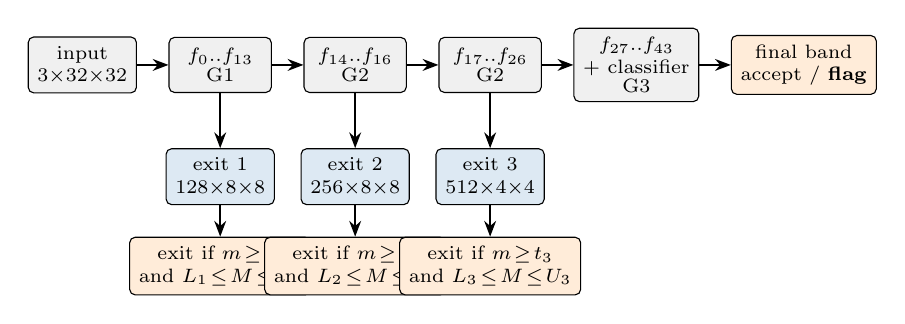
\begin{tikzpicture}[
  blk/.style={draw, rounded corners=2pt, fill=gray!12, minimum height=7mm, minimum width=13mm, font=\scriptsize, align=center},
  head/.style={draw, rounded corners=2pt, fill=cours!15, minimum height=6mm, minimum width=13mm, font=\scriptsize, align=center},
  dec/.style={draw, rounded corners=2pt, fill=orange!15, minimum height=6mm, minimum width=13mm, font=\scriptsize, align=center},
  arr/.style={-{Stealth[length=2mm]}, thick}, node distance=4mm]
  \node[blk] (in) {input\\$3{\times}32{\times}32$};
  \node[blk, right=of in] (b1) {$f_0..f_{13}$\\[-1pt]G1};
  \node[blk, right=of b1] (b2) {$f_{14}..f_{16}$\\[-1pt]G2};
  \node[blk, right=of b2] (b3) {$f_{17}..f_{26}$\\[-1pt]G2};
  \node[blk, right=of b3] (b4) {$f_{27}..f_{43}$\\+ classifier\\[-1pt]G3};
  \node[dec, right=of b4] (d4) {final band\\accept / \textbf{flag}};
  \draw[arr] (in) -- (b1); \draw[arr] (b1) -- (b2); \draw[arr] (b2) -- (b3); \draw[arr] (b3) -- (b4); \draw[arr] (b4) -- (d4);
  \node[head, below=7mm of b1] (h1) {exit 1\\$128{\times}8{\times}8$};
  \node[head, below=7mm of b2] (h2) {exit 2\\$256{\times}8{\times}8$};
  \node[head, below=7mm of b3] (h3) {exit 3\\$512{\times}4{\times}4$};
  \draw[arr] (b1) -- (h1); \draw[arr] (b2) -- (h2); \draw[arr] (b3) -- (h3);
  \node[dec, below=4mm of h1] (d1) {exit if $m\!\ge\!t_1$\\and $L_1\!\le\!M\!\le\!U_1$};
  \node[dec, below=4mm of h2] (d2) {exit if $m\!\ge\!t_2$\\and $L_2\!\le\!M\!\le\!U_2$};
  \node[dec, below=4mm of h3] (d3) {exit if $m\!\ge\!t_3$\\and $L_3\!\le\!M\!\le\!U_3$};
  \draw[arr] (h1) -- (d1); \draw[arr] (h2) -- (d2); \draw[arr] (h3) -- (d3);
\end{tikzpicture}
\caption{Final early-exit VGG16-BN (exits 13, 16, 26). $m$ = margin, $M$ = maximum logit; G1/G2/G3/HEADS =
fault groups.}
\end{figure}

\begin{itemize}
  \item \textbf{Main result:} SDC $13.4\,\%$ (plain) $\to$ $\mathbf{0.223\,\%}$; $93.1\,\%$ of harmful runs
        detected, FPR $0.08\,\%$; accuracy under faults $80.0 \to 87.4\,\%$; $60.5\,\%$ FLOPs saved.
  \item \textbf{Per bit ($k=1$):} bit 30 SDC $36.4\,\%$ plain, $18.5\,\%$ MENDNet, $\mathbf{0.10\,\%}$ ours;
        residual SDC mostly bit 26 ($\approx0.5\,\%$ for every method).
  \item \textbf{Robustness:} 5 exit configurations all SDC $0.12$--$0.22\,\%$; 3 head seeds SDC
        $0.211\pm0.011\,\%$.
  \item \textbf{Latency (batch 1, real early stopping):} CPU $11.4 \to 3.42$\,ms ($3.3\times$);
        A100 GPU $1.91 \to 1.37$\,ms ($1.4\times$).
 
\end{itemize}

\end{document}
